\chapter{State of the Art}

Text goes here.

Focus on multiprocessing models which focus on performance improvements.

\begin{itemize}
    \item Single source kernel: OpenCL, HIP.
    \item Language extensions for high level parallelism: OpenMP, OpenACC, SYCL, C++ AMP.
    \item Proprietary solutions: CUDA.
\end{itemize}

Other types of models which focus on scalability, but not covered \cite{survey_programming_models}:

\begin{itemize}
    \item Actor model
    \item MPI
\end{itemize}

\section{GPGPU}
The first documented case of computation on a graphics processor dates to June 1985, when Tim Van Hook implemented the world's first GPU ray-tracing on the Ikonas RDS-3000 \cite{ikonas}. Van Hook followed this up the next year with a paper on solid modelling with the Ikonas \cite{solid_modeling_ikonas}.

In August 1999, Kedem et al. \cite{unix_passwords_gpgpu} published a paper where they used experimental graphics engine PixelFlow to perform a brute force attack on Unix passwords. PixelFlow was a heterogeneous parallel machine used for high-speed and high-quality image generation. For their research, PixelFlow was setup with 18 SIMD arrays, each one with 8K processing elements (PE) for a total of 144K (147,456) PEs running at 100Mhz. The machine had some performance problems for this application due to the limited instruction set, which was focused on image computations. Due to this, the results were poorer than expected. It was calculated that the machine would be able to check all lowercase passwords (28.9\% of passwords at the time) in 3.19 hours.

\begin{figure}[h]
    \centering
    
\includegraphics[width=0.5\textwidth]{img/voronoi.png}
    \captionsetup{justification=centering}
    \caption{Generalized Voronoi diagram computed interactively on PC (Credit: Hoff et al.)}
\end{figure}

Also in 1999, Hoff et al. \cite{voronoi_diagrams_gpgpu} managed to perform computations of generalized Voronoi diagrams using graphics accelerators, such as the NVIDIA TNT2, connected to a PC \cite{brief_history_gpgpu}, as opposed to the specialized hardware in the PixelFlow. This was achieved by using the OpenGL API \cite{opengl}. However, at that time GPUs were not programmable. The hardware exposed what is known as a Fixed Function Pipeline which the user could configure according to their needs. With that configuration, the GPU would execute a series of built in math functions which were focused on rendering, not on computation \cite{opengl_fixed_function_pipeline}.

Programmable GPUs did not come until 2001, as NVIDIA introduced GeForce series 3. This replaced the fixed functions in the previous model with programmable shaders which could be controlled by the developers \cite{nvidia_nfinitefx_pixel, nvidia_nfinitefx_vertex}. These features were, of course, aimed at game developers and 3D designers, but they also allowed for new applications of GPU technology.

Using a GeForce 3, Larsen and McAllister achieved the first matrix multiplication done on a GPU \cite{early_matrix_multiplication_gpgpu}. Their work had to be done by mapping the matrices into textures that could be manipulated with the OpenGL API. This textures would be transfered to the GPU, rendered and then copied back to CPU memory to be mapped again to a matrix format so results could be read. Incidentally, the resulting "matrix texture" would be shown on screen. There is no explicit mention of the use of programmable shaders in this work, however this would not have changed the study drastically as the fixed functions of the previous model could handle the operations required. The main problem Larsen and McAllister found was the 8 bit fixed point precision and saturation arithmetic used by the hardware. Saturation arithmetic, although very useful in graphics, makes it harder to design a higher precision fixed-point implementation.

Approximate simulations of natural phenomena were achieved on the GPU by Harris et al. \cite {physics_simulations_gpgpu}. This included interactive visualizations of convection, reaction-diffusion and boiling. As the end effect of the simulation was to display visuals, this application had the advantage that data did not need to be transferred back to the CPU once results were computed. Again, during these experiments the most problematic aspect was the precision of the fixed-point operations. This contributed to more difficult programmability and arithmetic errors. During this work, the researchers exploited the programming capabilities of the GeForce 3 and, at the time, newly released GeForce 4. ATI had also released a programmable GPU, in the form of the Radeon 8500, which promised to add more power to the simulations, however the system was not ported to it at the time of publication. 

In late 2002, after seeing the growing trend in general purpose computation on GPUs, Harris coined the term GPGPU, an acronym for "General Purpose computing on Graphics Processing Units" \cite{brief_history_gpgpu}. GPGPU.org, a website dedicated to news on GPGPU research, would go live August 2003.

DirectX 9 (DX9) introduced the Shader Model 2.0 and with it support for floating-point operations. ATI released the Radeon 9700 PRO in July 2002, the first DirectX 9 capable graphics card \cite{ati_9700_pro}, NVIDIA followed up with their own DX9 GPU, the GeForceFX, in January 2003 \cite{geforcefx}. \cite{photon_mapping_gpgpu}

\section{OpenCL}

\begin{figure}[h]
    \centering
    
\includegraphics[width=0.5\textwidth]{img/opencl-logo.png}
    \captionsetup{justification=centering}
    \caption{OpenCL logo (Credit: Khronos Group)}
\end{figure}

OpenCL \cite{opencl_spec} is an open industry standard for programming a heterogeneous collection of CPUs, GPUs and other discrete computing devices organized into a single platform. It provides a framework for parallel programming and includes a language, API, libraries and a runtime system to support software development. By leveraging OpenCL, an application can use a host and one or more OpenCL devices as a single heterogeneous parallel computer system.

The framework is comprised by the following components:
\begin{itemize}
    \item \textbf{Platform layer}: allows the host program to create contexts and discover OpenCL devices and their capabilites.
    \item \textbf{Runtime}: allows the host program to manipulate contexts one they have been created.
    \item \textbf{Compiler}: creates program executables that contain OpenCL kernels. Depending on the capabilities of a device, the compiler may build executables from either OpenCL C source strings, the SPIR-V intermediate language, or device-specific program binary objects. Some implementations may support other kernel languages or intermediate languages.
\end{itemize}

OpenCL C \cite{opencl_c_spec} is the programming language provided by the standard to write kernels that execute on an OpenCL device. OpenCL C is based on the \textit{ISO/IEC 9899:1999 - Programming languages - C} specification (also referred to as C99) \cite{c99}, with the addition of some \textit{ISO/IEC 9899:2011 - Information technology - Programming languages - C} specification (also referred to as C11) \cite{c11} features, plus some extensions and restrictions to support parallel kernels.

This dedicated kernel language allows the developer to write a single code base and execute it in different devices. This ensures the \textit{functional} portability of code across devices, eliminating the need for applications to be re-coded on a per-device or per-programming toolkit basis \cite{performance_portability_2013}. However, portability issues may still arise if the hardware supports different versions of the standard. In addition, there can also be issues in terms of performance portability due to architecture differences and compiler optimizations available on each platform \cite{performance_portability_2013, performance_portability_2019, performance_portability_2020}. For maximum performance, some tweaking of the source code may still be necessary depending on which device is being targeted \cite{optimizing_opencl_fpga_integer, optimizing_opencl_fpga_automata}.

SPIR-V is an intermediate language which is also supported as an input language for OpenCL. Instead of distributing and ingesting OpenCL C in the host, developers can precompile their kernels into SPIR-V, allowing for faster kernel load times and avoiding directly exposed source code \cite{spir_overview}. While SPIR-V is also supported by the Vulkan \cite{vulkan} graphics API, it uses a different execution mode of the language (\textbf{GLCompute} versus \textbf{Kernel} for OpenCL), so compute codes are not interchangable \cite{spir_spec}. Another caveat is that SPIR-V support is only mandatory for OpenCL 2.1 and 2.2 devices, support was made optional for OpenCL 3.0 devices \cite{opencl_spec}.

Today, OpenCL is at the forefront of heterogeneous architecture programming. Seventeen different companies (including Apple, Intel, AMD and NVIDIA) distribute products conforming to the standard \cite{opencl_conformant_companies}. This allows an OpenCL kernel to run on the majority of hardware available on the market, including CPUs, GPUs, FPGAs and more.

\begin{figure}[ht]
    \centering
    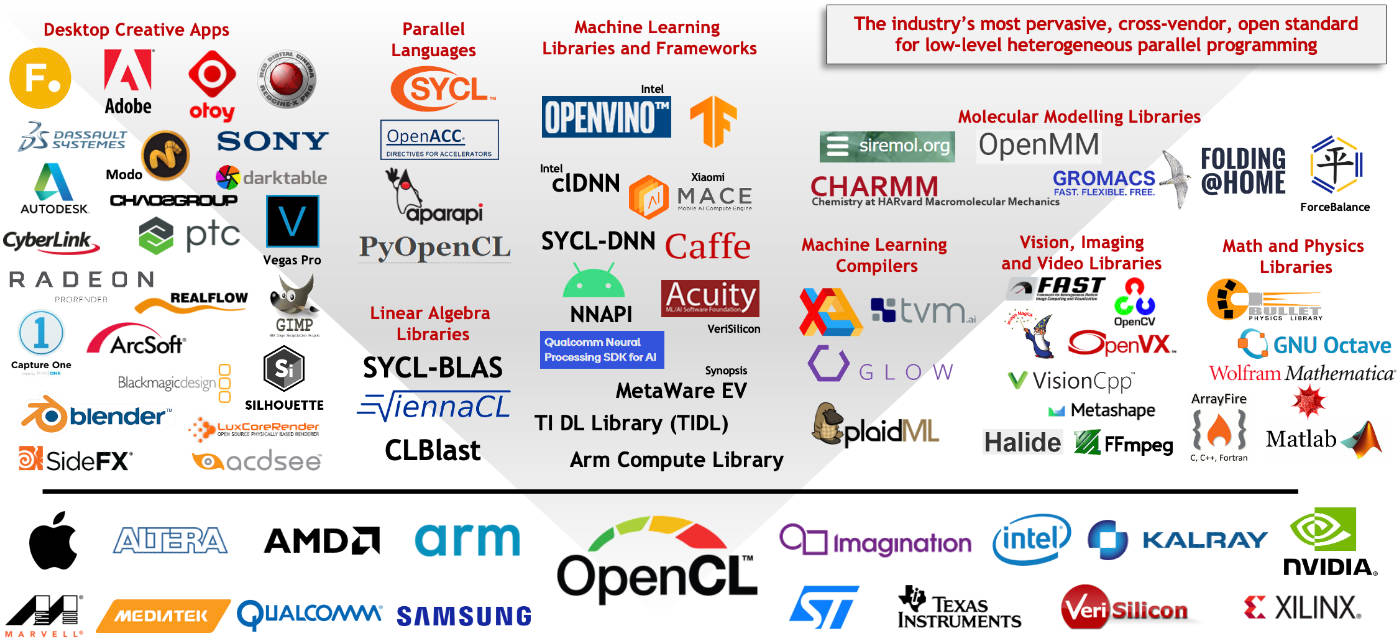
\includegraphics[width=\textwidth]{img/opencl-accelerated-apps.png}
    \captionsetup{justification=centering}
    \caption{OpenCL accelerated applications (Credit: Khronos Group)}
\end{figure}

Due to its popularity, a significant amount papers have been published looking into different types of extensions on the framework. We will focus on the extensions that are particularly relevant to our work. Section \ref{sub-sect:abstraction-layers} covers abstraction layers on top of OpenCL and section \ref{sub-sect:kernel_scheduling} covers kernel scheduling algorithms.

\subsection{Abstraction Layers} \label{sub-sect:abstraction-layers}
Even though OpenCL simplifies a big part of heterogeneous systems programming by providing a common API across devices, it still is a complex task. 
The articles presented in this section focus on simplifying the problem further by adding an abstraction layer on top of OpenCL.

In EngineCL \cite{enginecl}, a new object-oriented API is introduced. The EngineCL class provides a higher level view of the OpenCL context and management of the available devices. The engine in turn uses a Program object which internally manages all the data transfers between the device buffers, the user only needs to provide host input and output buffers, as well as the kernel arguments in order to begin execution. In addition, multiple devices can be used during a single run, the scheduling of which is handled by a Scheduler object. Different scheduling strategies are tested by the paper, with the best results achieved by the HGuided algorithm. HGuided is a dynamic algorithm which starts by assigning big block sizes to all devices and reducing the size of subsequent ones as the execution progresses. This reduces data transfer and synchronization overhead while allowing devices to finish simultaneously towards the end of the execution.

A different approch is presented by FluidiCL \cite{fluidicl}, where the OpenCL API is maintained but implemented in such a way that the user can treat multiple devices as a single entity. Thus, it is very easy to adapt an existing OpenCL application to run using FluidiCL, as all function calls are maintained. The paper considers the implementation running on an experimental system with a single GPU and CPU. At the time of setup, both kernel compilation and buffer writes are broadcasted to both devices. That is, the kernel is compiled for both and, likewise, the input data is transferred to the both of their buffers. When the execution starts, the GPU starts running the kernel with a decreasing order of work-group IDs, meanwhile the CPU executes smaller subkernels in increasing order of work-group IDs. At some point, when the work-groups IDs handled by both cross over, the work is finished and the results are merged on the GPU.

\subsection{Kernel Scheduling} \label{sub-sect:kernel_scheduling}
Multiple different techniques are discussed in order to optimize the scheduling of the kernels on the devices available on the platform. The overall objective always being minizing the turnaround time of a kernel or group of kernels.

\cite{transparent_cpu_gpu_collaboration} proposes the SKMD (Single Kernel Multiple Devices) system, where the workload of a single kernel can be split among all the available devices. At runtime, a partitioning algorithm will determine how to make this split, based on memory access pattern analysis of the kernel and previous profiling data. An effective partitioning makes sure that the performance improvements outweigh the overhead of extra memory transfers to the different devices. 

Machine learning is an alternative used to forgo the need of profiling the kernels before scheduling. \cite{smart_multitasking_scheduling} achieves this by implementing a model to predict the kernel speedup on a particular device based on static analysis of the code. Also, instead of focusing on a single kernel, it manages scheduling of multiple kernels, possibly belonging to different applications. A very similar approach is also proposed by \cite{load_balance_model_opencl_integrated_cluster}.

\section{OpenMP \& OpenACC}
In this section we will tackle OpenMP and OpenACC in conjunction as they take very similar approaches.

Both projects are composed of a library and set of compiler directives that provide a model for parallel programming across different architectures. Support is provided for the C, C++ and Fortran languages. The directives extend the languages with useful constructs for parallelizing applications. Further control of the runtime environment is possible through the library \cite{openmp_spec, openacc_spec}.

OpenMP and OpenACC allow for quick adaptation of existing single threaded code into a parallel execution model. This work requires a compiler which supports the standard, meaning that it is able to handle the directives and generate multithreaded code automatically. 

Up until version 4.0, OpenMP only allowed for this code to be compiled for and executed on the CPU. Version 4.0 (2013) introduced offloading of the parallel code to other devices like GPUs or FPGAs \cite{openmp_gpu_support}. Meanwhile OpenACC focused on heterogeneous computing and accelerator offloading from the start \cite{openacc_initial_spec}, also treating the multicore CPU itself as a device.

\cite{openmp_vs_openacc} provides a comparison of both programming models in terms of programmability and expressiveness. Here the authors denote the differences between OpenMP and OpenACC when implementing common parallel programming patterns targeting accelerators. Overall, the resulting code and directives used are mostly equivalent, with OpenACC having a slight advantage thanks to providing accelerator support since its inception. In terms of programmer effort, there is no significant difference. In terms of performance however, \cite{cuda_openacc_openmp_performance} shows that the code generated by OpenACC is able to utilize more memory bandwidth and thus perform better than OpenMP, specially when using a naive approach. Still, both approaches fall behind a pure CUDA kernel.

Finally, the possibility to use both models at the same time exists. Works like \cite{openmp_openacc_multigpus} exploit parallelism on the CPU with OpenMP to schedule code to run on multiple GPUs. \cite{openmp_openacc_molecular_docking} also leverages this hybrid approach to run kernels which are more GPU friendly on the GPU using OpenACC while running less friendly kernels with OpenMP CPU parallelization. 

\section{CUDA}

\section{HIP}

\section{SYCL}
\subsection{Celerity}

\section{Kokkos}
\cite{kokkos}

\section{C++ AMP}
Appears dead. Stack overflow post by one of the authors \url{https://stackoverflow.com/a/38604348/7983805}


\section{Standalone works}

Here goes what we don't where to put. Also may be deleted entirely.

\subsection{Kernel scheduling}

\cite{dynamic_self_scheduling} presents HDSS, a Heterogeneous Dynamic Self Scheduler, which can reschedule at runtime how the workload is partitioned across the devices. This is achieved by a two phase approach. First, in the adaptive phase, the scheduling algorithm will measure the relative performance across devices by dispatching increasing block sizes. Once an accurate performance approximation for each device is calculated, the completion phase starts. Here the scheduler assigns the largest possible block size to each device, according to its calculated performance, in order to minimize data transfer overhead. The approach presented not only keeps all devices busy during the entire execution, but also fully utilizes them by providing appropiate block sizes. 
